\section{Experimental results}

The motor setup used in the experiments is shown in Fig. \ref{Fig:M3-setup}. A PM motor is on the left and a synchronous reluctance motor (SyRM) on the right. The SyRM was used as a load machine, which allowed the compensator performance measurements under different load conditions. A brushless resolver, with $10$ kHz excitation signal frequency, was connected to the PM motor and was used for measuring the speed. The PM motor parameters are listed in Table \ref{Tbl:MS4887}.

%Performance data was collected from two different sources. A brushless resolver, with $10$ kHz excitation signal frequency, was connected to the PM motor and was used for measuring the speed. Respectively, a DATAFLEX 22/100 torque transducer, connected to the motor shafts, was used for measuring torque. The PM motor parameters are listed in Table \ref{Tbl:MS4887}.

\begin{figure}[htb] 
    \centering
    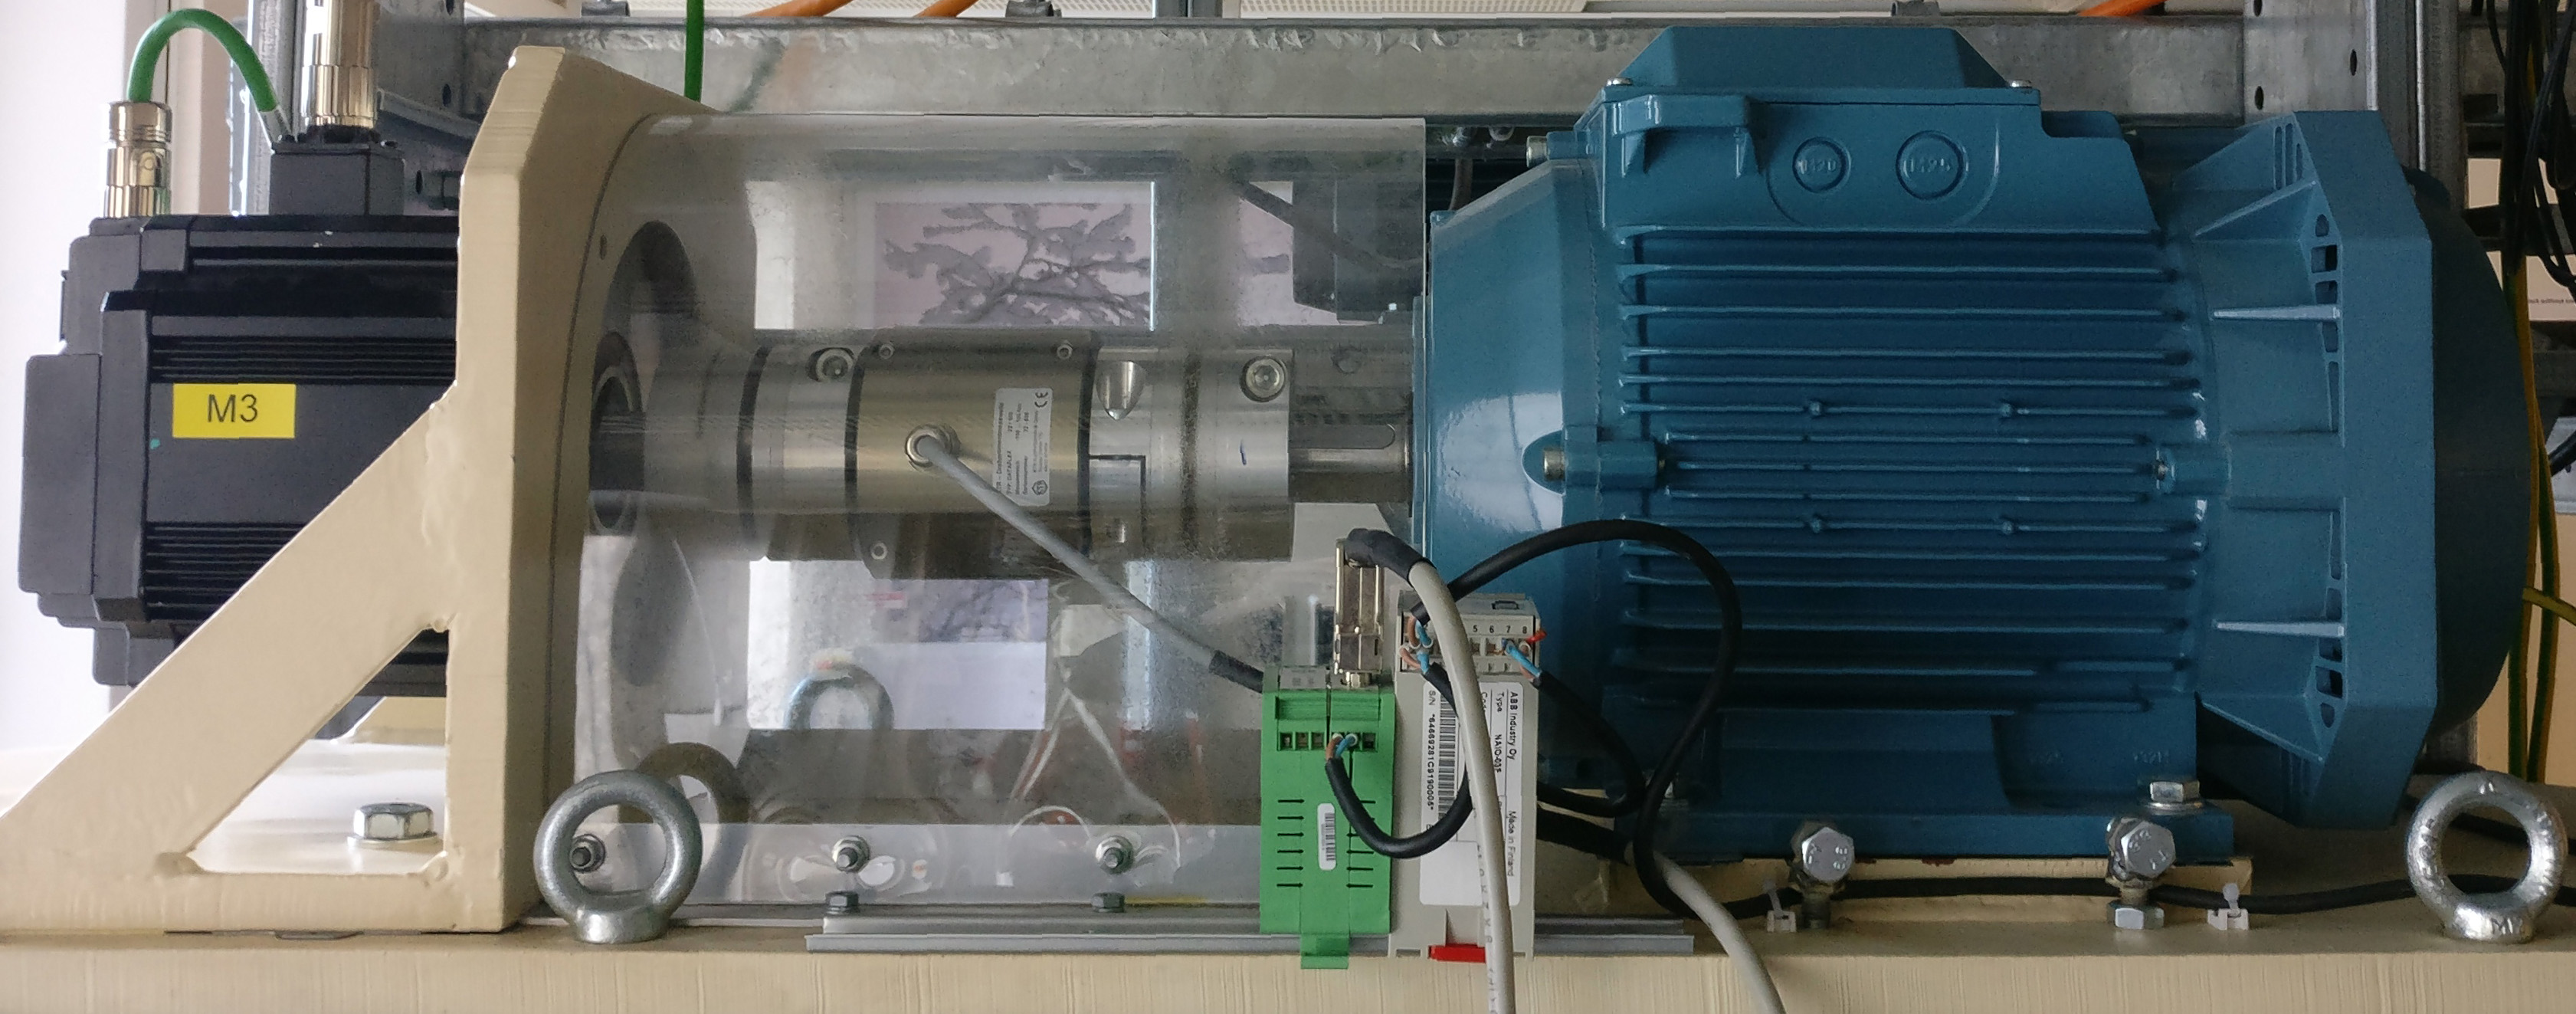
\includegraphics[width=1.0\textwidth]{images/M3-setup.jpg}
    \caption{Main motor setup used for the experiments}
    \label{Fig:M3-setup} 
\end{figure}

% Instead of evenly distributing the operating points, the selection
% is based on a idea to test the compensator on: no-load, low-load, mid-load and high-load conditions. For this reason, the different loads were selected to be: 0%, 10%, 50%, 80% of nominal torque of the other motor???

Experimental results were collected and evaluated in a similar manner to the simulation results. Three measurements with all control methods were taken in each operating point and then these results were compared. The performance comparison was conducted comparing amplitudes of speed harmonics and using the SRF \eqref{eq:ripple-factor} measure.
%\begin{table}[ht]
%\caption{MS4887 motor nameplate values}
%\centering
%\begin{tabular}[t]{lccc}
%\hline
%Description & Symbol & Value  & Unit\\
%\hline
%Nominal current   & $I_N$      & 18.1  & A\\
%Nominal voltage   & $U_N$      & 195.1 & V\\
%Nominal frequency & $f_N$      & 133.3 & Hz\\
%Nominal speed     & $\omega_N$ & 2000  & rpm\\
%Nominal power     & $P_N$      & 6     & kW\\
%Nominal torque    & $T_N$      & 28.6  & Nm\\
%Number of poles   & $N_p$      & 8     & no.\\
%\hline
%\label{Tbl:MS4887}
%\end{tabular}
%\end{table}%

\subsection{Measurement considerations}

Compensation performance was tested in different load conditions. The load machine was used to produce loads corresponding 0\%, 10\%, 50\% and 80\% of the nominal torque of the PM machine. The speed reference was kept at constant $60$ rpm.

%The servomotor in second setup was not connected to any load. Hence, only no-load tests were possible. However, various speeds were tested when verifying the results to provide additional information.

% offsets can also drift
During the drive startup, current offsets are automatically identified and removed. This process is performed automatically after every drive startup. Therefore, the Q-learning and ILC measurements taken on different times, are not necessarily directly comparable, since there can be variation between harmonics. Especially, the first harmonic induced by current offsets may be slightly different. For this reason, the ILC and Q-learning measurements are visualized separately. PI speed control measurements were taken twice in conjunction with compensator measurements. Hence, PI speed control measurements allow calculation of reduction ratio, which makes it possible to compare compensation methods rigorously.

It was also found that there is misalignment between the motor shafts, which leads to mechanical oscillations visible in the Fourier spectrum. The frequency of these oscillations seemed to be different from the harmonics being studied.

The torque transducer visible in Fig. \ref{Fig:M3-setup} was planned to be used for measuring torque. Unfortunately, the readings were found to drift and torque measurements had to be discarded as these cannot be considered to be reliable. Therefore, only speed measurements are used for making conclusions. On the bright side, the speed signal was found to be more reliable than torque signal in the chapter \ref{Results with fine tuned compensators}. For this reason, the torque measurements can be considered to be redundant and these could have been only used for verification. Now the verification of results is done by testing the compensation with supplementary motor setup.

%Number of poles can be determined by calculating $p = (120 * 133.3)/2000 \approx 8$. Hence, MS4887 has four pole pairs. This information allows calculation of fundamental frequency. With 60 rpm, the $f_{n60} = (60 / 60) * 4 = 4 Hz$. With ten times higher speed, the fundamental frequency is obviously $40Hz$.

\subsection{ILC measurements}
When testing ILC, the tuning strategy was to find a maximum value for gain $\Phi$, which still keeps the system stable, as this maximizes the compensation performance. The $\alpha$ and $\Gamma$ gains were adjusted as little as possible between different operating points in order to make it easy to see effects of $\Phi$ adjustment. However, a higher $\alpha$ value was used, if this made it possible to use higher $\Phi$ gain value. The gain $\Gamma$ was initially set low to make it possible to keep a higher $\Phi$ gain value at the cost of slower learning rate. The gains used in the experiments are listed in Table \ref{tab:60rpm}.
\begin{table}[htb]
\caption{ILC gains used in $60$ rpm measurements}
\centering
\begin{tabular}{lcccccccr}
\toprule
\multicolumn{4}{c}{Motoring} & \multicolumn{4}{c}{Generating}\\
\cmidrule(r){2-5} \cmidrule(r){6-9}
Load         & 0\% & 10\% & 50\% & 80\%   & 0\%    & 10\% & 50\% & 80\% \\
\midrule
$\alpha$     & 0.15 & 0.15 & 0.15 & 0.25   & 0.10  & 0.10 & 0.10 & 0.10 \\
$\Gamma$     & 1.0  & 1.0  & 1.0  & 1.0    & 1.0   & 1.0  & 1.0  & 1.0 \\
$\Phi$       & 4.75 & 3.0  & 2.8  & 1.25   & 3.0   & 2.9  & 3.0  & 3.0 \\
\bottomrule
\label{tab:60rpm}
\end{tabular}
\end{table}


%ILC gains have a direct effect on how well the ILC compensates. Higher gains usually produce better compensation results, but these also drive the system closer to instability. Thus, the gains cannot be set arbitrarily high and therefore appropriate gains must be searched for. During testing, it was found that measurement noise has direct effect, how high gains can be selected. In simulator, where noise does not exist unless explicitly generated, it was possible to use much higher gains than it was in practice. It was found that the gains were often the bottleneck for the ILC, as the noise coming from the speed measurements did not allow to set enough high gains for proper compensation.

It can be observed from Table \ref{tab:60rpm} that the compensator behaviour was not identical in motoring and generating modes. The generating mode was easier for the compensator to handle, since gains could be kept almost identical between different operating points, whereas the motoring mode required more re-tuning. The control algorithms in both operation modes are similar, but not identical. Hence, software differences may provide an answer to different behaviour, as well as, differences in the machine dynamics between motoring and generating modes. Nevertheless, the gains could not be kept the same in all operating points, even when considering only one operation mode. Therefore, a gain scheduling scheme would be needed in order to be able to use ILC in different operating points automatically. Without gain scheduling, the system can become unstable when operating point is changed. Another solution to the problem is to use gain values that work in the most demanding operating point, but then the compensation performance is compromised in less demanding conditions.

% 0%  PI-SRF = 0.143, ILC-SRF = 0.143
% 10% PI-SRF = 0.185, ILC-SRF = 0.194
% 50% PI-SRF = 0.555, ILC-SRF = 0.340
% 80% PI-SRF = 0.968, ILC-SRF = 0.837

At low load conditions, the compensation is almost nonexistent. With two decimal accuracy, the PI and ILC SRF is $0.14$\% at 0\% load. The same applies, when the load is increased to 10\%. The SRF is $0.19\%$ with PI and ILC. When load is increased to 50\% level, the pulsations become more visible, which makes identification and compensation easier. The compensator reduces SRF from $0.56 \%$ to $0.34 \%$. At 80\% load, the ILC manages to reduce SRF from $0.97\%$ to $0.84\%$. Compensation performance is worse at 80\% load than at 50\% load, even when the magnitude of pulsations is greater. One possible reason for worse performance are the gain values that do not allow ILC to inject enough high correction value to the q-axis current reference. Another possible explanation is the altered type of torque and speed pulsations. Under heavy load, noninteger harmonics become greater due to non-ideal load mechanism when DC generator is excited for loading purposes \cite{ILC:Book2009}. The induced noninteger harmonics cannot be compensated by ILC \cite{ILC:2005, ILC:Book2009}, which results to worse overall performance.
\begin{figure}[p] 
    \centering
    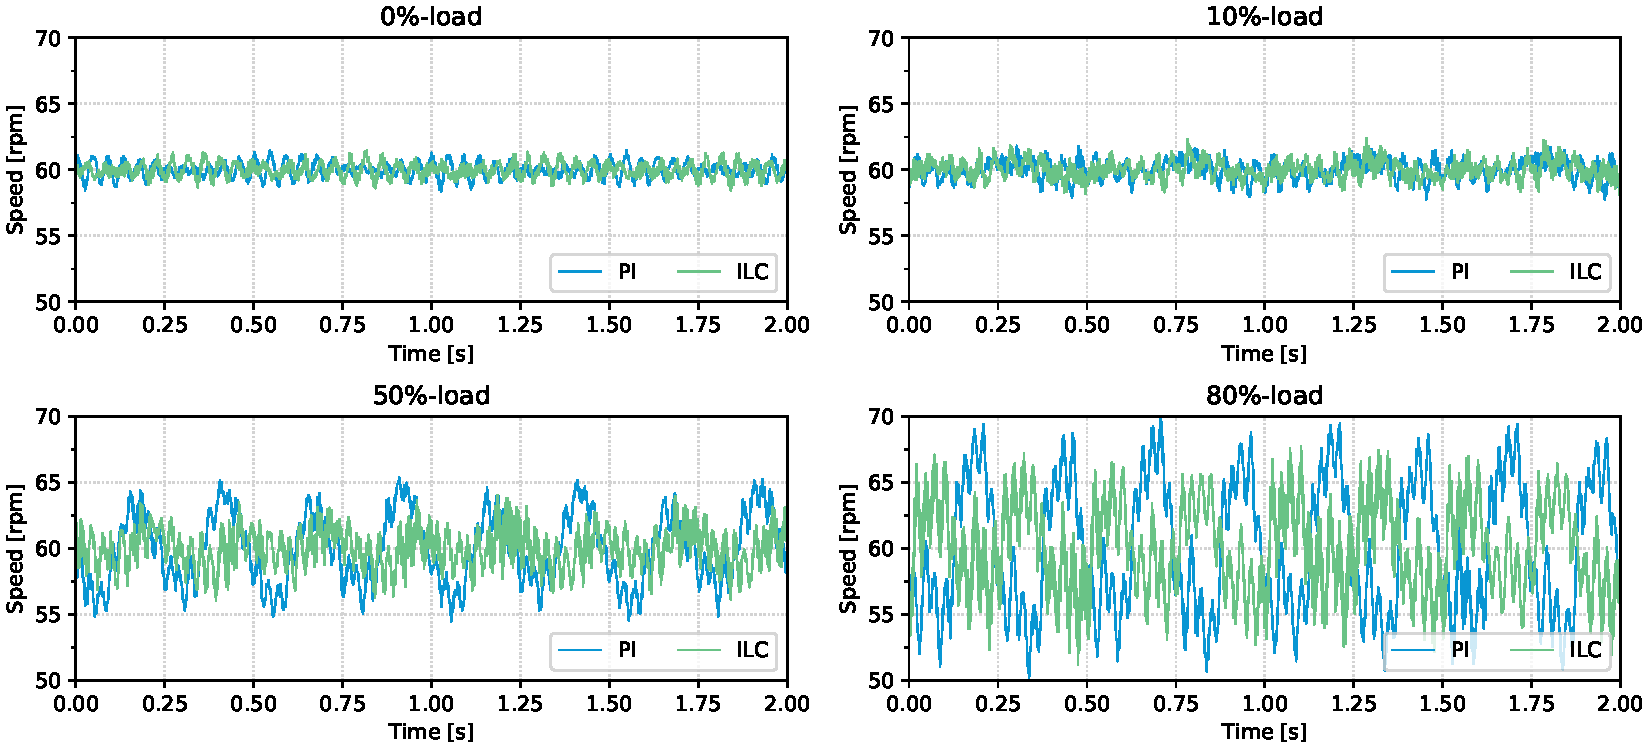
\includegraphics[width=1.0\linewidth]{images/PI-ILC-comparison-time-domain.pdf} 
    \caption{Speed pulsations encountered with PI control getting reduced when ILC based compensator is used at 60 rpm speed}
    \label{Fig:experiment-ilc-speed}
\end{figure}

\begin{figure}[p] 
    \centering
    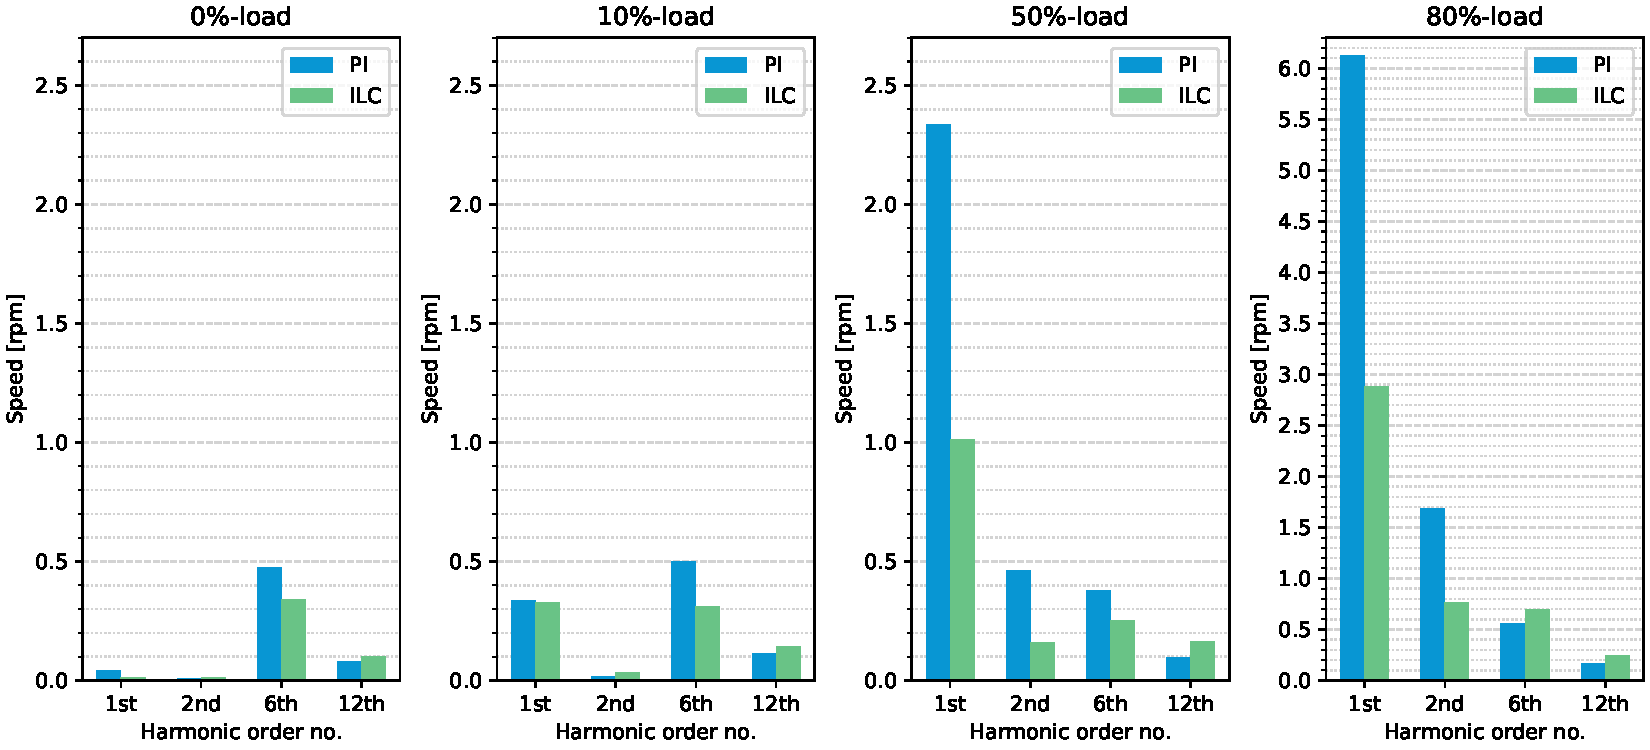
\includegraphics[width=1.0\linewidth]{images/PI-ILC-comparison-harmonics.pdf} 
    \caption{Speed harmonics with PI control and ILC at $60$ rpm speed}
    \label{Fig:experiment-ilc-harmonics-speed}
\end{figure}

%% Mention that method tries to reduce significant harmonics, thus often reducing the greatest harmonic as 
%% this has the greatest impact on the torque ripple
% The method can reduce the greatest harmonic at cost of increasing the others. 
The speed harmonics in Fig. \ref{Fig:experiment-ilc-harmonics-speed} are consistent with SRF measures. With 80\% load, the compensation performance is truly worse than with 50\% load. With 50\% load, the first compensated harmonic can be seen to be less than half of the original amplitude, wherease with 80\% load, it is roughly half of the original amplitude. At 0\% and 10\% loads, ILC manages to reduce disturbance harmonics only slightly in overall. However, the pulsations are also small with low loads. With higher loads the pulsations become more noticeable and ILC is able to reduce the harmonics significantly.

% 0%  PI-TRF = 198.241, ILC-TRF = 203.321.
% 10% PI-TRF = 413.079, ILC-TRF = 568.124
% 50% PI-TRF = 1149.953, ILC-TRF = 1115.944
% 80% PI-TRF = 1428.040, ILC-TRF = 1489.039





\subsection{Q-learning measurements}

% 0%  PI-SRF 0.153, ILC-SRF 0.175
% 10% PI-SRF 0.249, ILC-SRF 0.235
% 50% PI-SRF 0.500, ILC-SRF 0.434
% 80% PI-SRF 0.740, ILC-SRF 0.564
% Regardless of this, the compensator seems to compensate pulsation effectively. 
The measurements with the Q-learning based compensator were taken in a similar manner to the ILC measurements. The parameters used in measurements are the same as in the table \ref{Tbl:Q-params} with exceptions of $\lambda = 1$ and $k_\epsilon = 750$. The pulsation maximum $T_{max}$ was adjusted between different operating points. All other parameters were kept constant. The parameter $T_{max}$ value was set by testing few different values and then selecting the one producing the best results. In practice, values $0.01$, $0.02$ and $0.035$ were used. These values are unlikely to be ideal and better compensation results could be achieved with better value selection.

Figure \ref{Fig:experimentl-qlr-speed} shows measured speed with conventional PI speed control and Q-learning based compensator. It can be observed that speed pulsations are smaller at higher loads when Q-learning based compensator is used. Since speed pulsations are getting reduced, also torque pulsations must be getting smaller according to \eqref{Eq:transfer_function}. Therefore, it can be concluded that the method can compensate torque pulsations successfully.

Speed ripple factors were calculated in different operating conditions. With 0\% load, the SRF is $0.15\%$ with conventional PI speed control and $0.18\%$ when the compensator is used. Figure \ref{Fig:experimentl-qlr-speed} verifies the result of the ripple not getting reduced when the Q-learning based compensator is enabled at 0\% load. However, at 10\% load, the compensator is able to reduce the speed ripple slightly. With PI control, the SRF is $0.25\%$ and with Q-learning, it is $0.24\%$. Similarly to ILC, the ripple reduction is more significant at 50\% and 80\% loads when magnitude of pulsations is much greater than with lower loads. At 50\% load, the compensator reduces SRF from $0.50\%$ to $0.43\%$. Unlike to ILC, the ripple reduction is even greater when load is increased from 50\% to 80\%. At 80\% load, the SRF with PI is $0.74\%$ and with Q-learning it is $0.56\%$.

Figure \ref{Fig:experimentl-qlr-harmonics-speed} shows speed harmonics that were obtained by computing FFT from the speed measurements. In overall, the harmonics are congruent with the SRF measures. Disturbances are getting reduced in all studied operating points when compensation is used. Therefore, the compensator seems to be functioning properly.
\begin{figure}[p] 
    \centering
    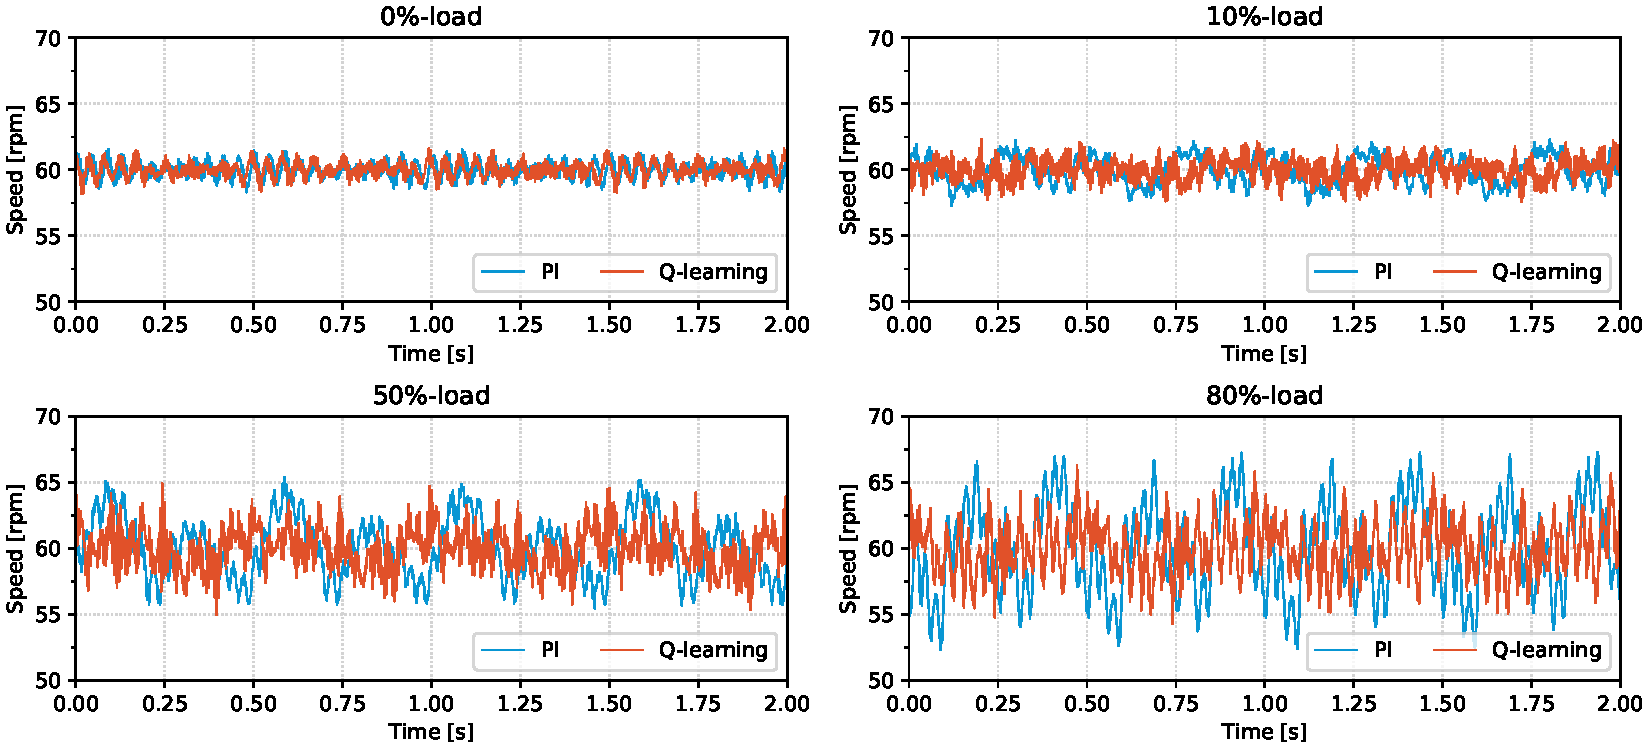
\includegraphics[width=1.0\linewidth]{images/PI-QLR-comparison-time-domain.pdf} 
    \caption{Speed pulsations encountered with PI control getting reduced when Q-learning based compensator is used at 60 rpm speed}
    \label{Fig:experimentl-qlr-speed}
\end{figure}

\begin{figure}[p]
    \centering
    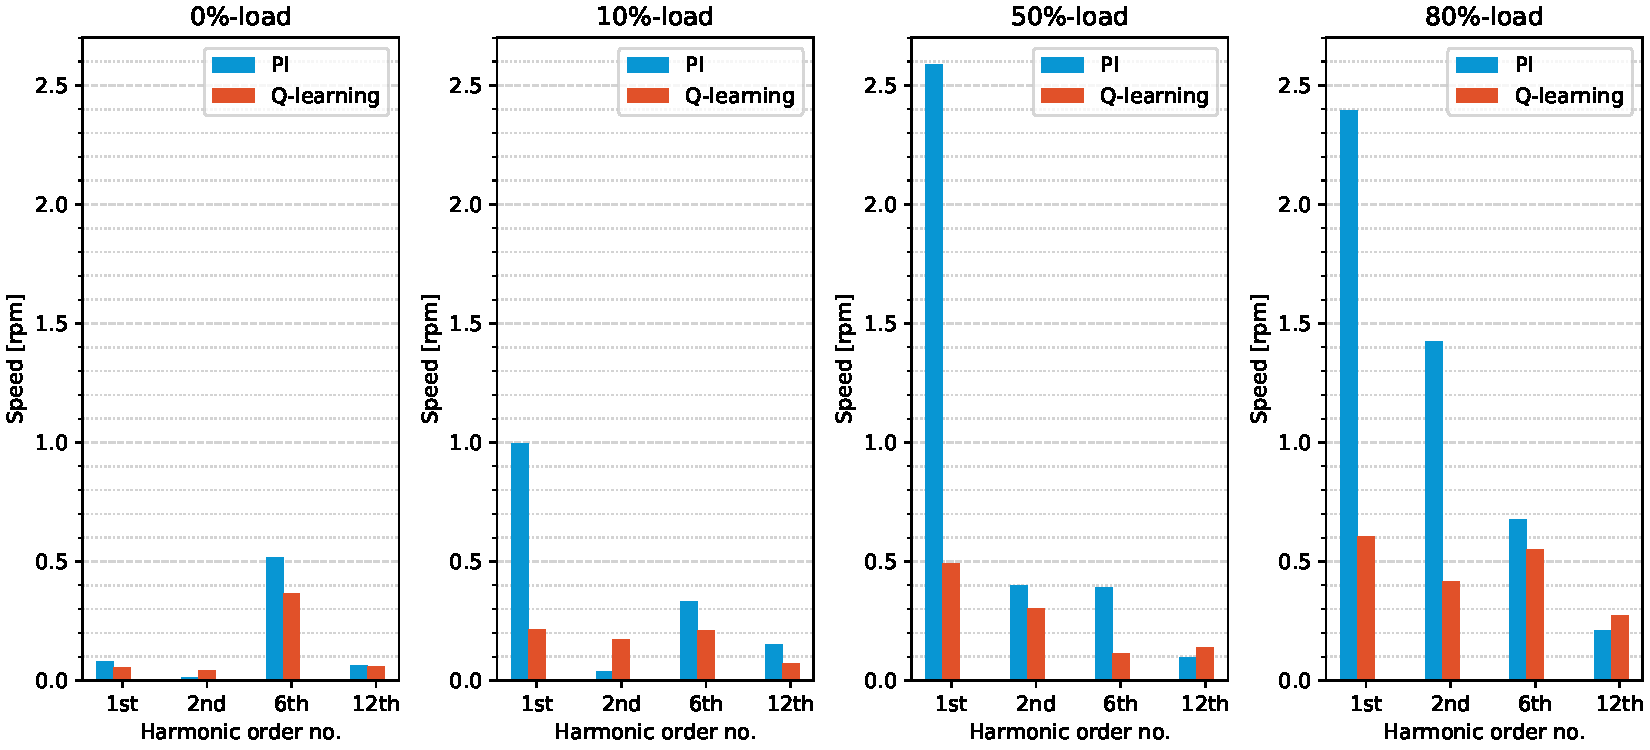
\includegraphics[width=1.0\linewidth]{images/PI-QLR-comparison-harmonics.pdf} 
    \caption{Speed harmonics with PI control and Q-learning at $60$ rpm speed}
    \label{Fig:experimentl-qlr-harmonics-speed}
\end{figure}
% PI-TRF,   QLR-TRF
% 239.420, 233.990
% 309.900, 328,300
% 490.400, 528,800
% 591.500, 737,099

\subsection{ILC and Q-learning performance evaluation}

% ILC - percent from original, reduction
%1.00
%1.05
%0.61
%0.86

% QLR
%1.15
%0.94
%0.87
%0.76

Table \ref{Tbl:reduction} shows reduction ratios that have been calculated from SRF measures. The ratios show how much smaller the ripple became when compensator was enabled. For example, reduction ratio for Q-learning at 10\% load is calculated as $0.235 / 0.249 = 0.94$. The ratio allows to conclude that the ripple became 6\% smaller when Q-learning based compensation was used.

According to reduction ratios, ILC and Q-learning based compensators should not be used if pulsations are minimial, since the ripple is not getting reduced. When pulsations become notable, then both compensators do reduce the ripple remarkably. ILC performs better at 50\% load region than Q-learning, but at 80\% load, the situation is opposite. ILC may get limited by gain values, which explains why Q-learning based compensator performs better at 80\% load. However, current reference injections made by ILC are more accurate than corrections done by Q-learning method, which explains better performance of ILC at 50\% load where it is not getting limited as much. ILC can inject any real value whereas Q-learning method uses quantized actions. Therefore, ILC can theoretically achieve better performance.
\begin{table}[htb]
\caption{Speed ripple reduction ratios with different loads}
\centering
\begin{tabular}[t]{lcccc}
\hline
Load & ILC & Q-learning\\
\hline
0\%   & 1.0   & 1.15\\
10\%  & 1.05  & 0.94 \\
50\%  & 0.61  & 0.87 \\
80\%  & 0.86  & 0.76 \\
\hline
\label{Tbl:reduction}
\end{tabular}
\end{table}%

\clearpage
